%9_central_limit_theorem
%notes for the course Probability and Statistics COMS10011
%taught at the University of Bristol
%Conor Houghton conor.houghton@bristol.ac.uk
%To the extent possible under law, the author has dedicated all copyright
%and related and neighboring rights to these notes to the public domain 
%worldwide. These notes are distributed without any warranty. 

\documentclass[11pt,a4paper]{scrartcl}
\typearea{12}
\usepackage{graphicx}
%\usepackage{pstricks}
\usepackage{listings}
\usepackage{color}

\newif\ifind
\indtrue

\lstset{language=C}
\usepackage{fancyhdr}
\pagestyle{fancy}
\lfoot{\texttt{coms10011.github.io}}
\lhead{COMS100011 9\_central\_limit\_theorem - Conor}
\begin{document}

\section*{9 The Central Limit Theorem}

\subsection*{The sum of two random variables}

Say we have two continuous random variables $X$ and $Y$, with density
functions $p_X(x)$ and $p_Y(y)$; consider working out the distribution for 
\begin{equation}
Z=X+Y
\end{equation}
Now the thing is that there is more than one value for $x$ and $y$
that gives $Z=z$. In fact $Z=z$ if $Y=z-x$ for any value of $x$ so
\begin{equation}
p_Z(z)=\int_{-\infty}^\infty {p_X(x)p_Y(z-x)dx}
\end{equation}
This calculation is called a \textbf{convolution}.

As a simple example consider $X$ and $Y$ both uniformly distributed
over $[0,1]$:
\begin{equation}
p_X(x)=\left\{\begin{array}{ll}1:x\in[0,1]\\0:\mbox{otherwise}\end{array}\right.
\end{equation}
with $p_Y(y)$ the same. Now $Z=X+Y$ has the distribution
\begin{equation}
p_Z(z)=\int_{-\infty}^\infty {p_X(x)p_Y(z-x)dx}
\end{equation}
where the integrand is zero unless $x$ and $z-x$ are both inside the
interval zero to one. Now, the first contraint, $x\in [0,1]$ is easy
but the second one depends on $z$. If $z<0$ then $z-x$ is always
negative and $p_Y(z-x)=0$. If $z>2$ then $z-x>1$ and again
$p_Y(z-x)=0$. If $z\in [0,2]$ there are two cases, if $z<1$ then $x$
then $z-x>0$ for $x\in [0,z]$, otherwise if $z>1$ then $z-x<1$ in $x\in
[z-1,1]$. Lets do the two cases separately, for $z\in [0,1]$:
\begin{equation}
p_Z(z)=\int_0^z dx=z
\end{equation}
and for $z\in (1,2]$
\begin{equation}
p_Z(z)=\int_{z-1}^1dx=1-(z-1)=2-z
\end{equation}
Putting it all together we get
\begin{equation}
p_Z(z)=\left\{\begin{array}{ll} z&z\in [0,1]\\2-z& z\in [1,2]\\0&\mbox{otherwise}\end{array}\right.
\end{equation}

\subsection*{The sum of two Gau\ss{}ians}

Next lets consider the sum of two Gau\ss{}ians, $X\sim
\mathcal{N}(\mu_x,\sigma_x^2)$ and $Y\sim
\mathcal{N}(\mu_Y,\sigma_Y^2)$. Calculating the distribution of $Z=X+Y$ would be difficult since it involves the integral
\begin{equation}
p_Z(z)=\frac{1}{2\pi\sigma_X^2\sigma_Y^2}
\int_{-\infty}^\infty e^{-(x-\mu_X)^2/2\sigma_X^2-(z-x-\mu_Y)^2/2\sigma_Y^2}dx
\end{equation}
We aren't going to attempt that, but we will quote the result: the sum is also a Gau\ss{}ian:
\begin{equation}
Z\sim \mathcal{N}(\mu_X+\mu_Y,\sigma_X^2+\sigma_Y^2)
\end{equation}

\subsection*{The central limit theorem}

Let $\{X_1,X_2,\ldots,X_n\}$ be a set of random variables. A set of
random variables is called \textbf{independent identically distributed},
usually abbreviated to i.i.d., if the variables all have the same
probability density, say $p_X(x)$ and are independent. Let $\mu$ and
$\sigma^2$ be the mean and variance of that probability density. Now
consider the \textbf{sample mean}:
\begin{equation}
S_n=\frac{X_1+X_2+\ldots+X_n}{n}
\end{equation}
If you were estimating the mean for $X$ this is the value you would
measure if you took $n$ independent samples. Now the central limit
theorem stats that for $n$ approaching infinity
\begin{equation}
U_n=\sqrt{n}\left(\frac{S_n-\mu}{\sigma}\right) \sim \mathcal{N}(0,1)
\end{equation}

As an example, consider the uniform distribution example we looked
before; in Fig.~\ref{fig_const} we plot $U_n$ for different $n$. We
see that it very quickly comes to resemble a Gau\ss{}ian distribution.

\begin{figure}[tb]
\begin{center}
% GNUPLOT: LaTeX picture with Postscript
\begingroup
  \makeatletter
  \providecommand\color[2][]{%
    \GenericError{(gnuplot) \space\space\space\@spaces}{%
      Package color not loaded in conjunction with
      terminal option `colourtext'%
    }{See the gnuplot documentation for explanation.%
    }{Either use 'blacktext' in gnuplot or load the package
      color.sty in LaTeX.}%
    \renewcommand\color[2][]{}%
  }%
  \providecommand\includegraphics[2][]{%
    \GenericError{(gnuplot) \space\space\space\@spaces}{%
      Package graphicx or graphics not loaded%
    }{See the gnuplot documentation for explanation.%
    }{The gnuplot epslatex terminal needs graphicx.sty or graphics.sty.}%
    \renewcommand\includegraphics[2][]{}%
  }%
  \providecommand\rotatebox[2]{#2}%
  \@ifundefined{ifGPcolor}{%
    \newif\ifGPcolor
    \GPcolorfalse
  }{}%
  \@ifundefined{ifGPblacktext}{%
    \newif\ifGPblacktext
    \GPblacktexttrue
  }{}%
  % define a \g@addto@macro without @ in the name:
  \let\gplgaddtomacro\g@addto@macro
  % define empty templates for all commands taking text:
  \gdef\gplbacktext{}%
  \gdef\gplfronttext{}%
  \makeatother
  \ifGPblacktext
    % no textcolor at all
    \def\colorrgb#1{}%
    \def\colorgray#1{}%
  \else
    % gray or color?
    \ifGPcolor
      \def\colorrgb#1{\color[rgb]{#1}}%
      \def\colorgray#1{\color[gray]{#1}}%
      \expandafter\def\csname LTw\endcsname{\color{white}}%
      \expandafter\def\csname LTb\endcsname{\color{black}}%
      \expandafter\def\csname LTa\endcsname{\color{black}}%
      \expandafter\def\csname LT0\endcsname{\color[rgb]{1,0,0}}%
      \expandafter\def\csname LT1\endcsname{\color[rgb]{0,1,0}}%
      \expandafter\def\csname LT2\endcsname{\color[rgb]{0,0,1}}%
      \expandafter\def\csname LT3\endcsname{\color[rgb]{1,0,1}}%
      \expandafter\def\csname LT4\endcsname{\color[rgb]{0,1,1}}%
      \expandafter\def\csname LT5\endcsname{\color[rgb]{1,1,0}}%
      \expandafter\def\csname LT6\endcsname{\color[rgb]{0,0,0}}%
      \expandafter\def\csname LT7\endcsname{\color[rgb]{1,0.3,0}}%
      \expandafter\def\csname LT8\endcsname{\color[rgb]{0.5,0.5,0.5}}%
    \else
      % gray
      \def\colorrgb#1{\color{black}}%
      \def\colorgray#1{\color[gray]{#1}}%
      \expandafter\def\csname LTw\endcsname{\color{white}}%
      \expandafter\def\csname LTb\endcsname{\color{black}}%
      \expandafter\def\csname LTa\endcsname{\color{black}}%
      \expandafter\def\csname LT0\endcsname{\color{black}}%
      \expandafter\def\csname LT1\endcsname{\color{black}}%
      \expandafter\def\csname LT2\endcsname{\color{black}}%
      \expandafter\def\csname LT3\endcsname{\color{black}}%
      \expandafter\def\csname LT4\endcsname{\color{black}}%
      \expandafter\def\csname LT5\endcsname{\color{black}}%
      \expandafter\def\csname LT6\endcsname{\color{black}}%
      \expandafter\def\csname LT7\endcsname{\color{black}}%
      \expandafter\def\csname LT8\endcsname{\color{black}}%
    \fi
  \fi
  \setlength{\unitlength}{0.0500bp}%
  \begin{picture}(7600.00,5700.00)%
      \put(500,2600){\makebox(0,0)[r]{\strut{}$\mathbf{n=3}$}}%
      \put(858,440){\makebox(0,0)[r]{\strut{} 0}}%
      \put(858,1045){\makebox(0,0)[r]{\strut{} 0.15}}%
      \put(858,1651){\makebox(0,0)[r]{\strut{} 0.3}}%
      \put(858,2256){\makebox(0,0)[r]{\strut{} 0.45}}%
      \put(990,220){\makebox(0,0){\strut{}-5}}%
      \put(1543,220){\makebox(0,0){\strut{}-2.5}}%
      \put(2097,220){\makebox(0,0){\strut{} 0}}%
      \put(2650,220){\makebox(0,0){\strut{} 2.5}}%
      \put(3203,220){\makebox(0,0){\strut{} 5}}%
      \put(1100,2083){\makebox(0,0)[l]{\strut{}sum}}%
      \put(1100,1863){\makebox(0,0)[l]{\strut{}gaussian}}%
          \put(0,0){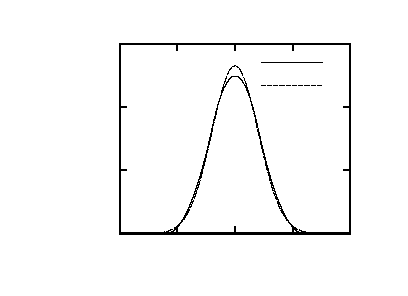
\includegraphics{conv_2}}%

      \put(4500,2600){\makebox(0,0)[r]{\strut{}$\mathbf{n=7}$}}%
      \put(4858,440){\makebox(0,0)[r]{\strut{} 0}}%
      \put(4858,1045){\makebox(0,0)[r]{\strut{} 0.15}}%
      \put(4858,1651){\makebox(0,0)[r]{\strut{} 0.3}}%
      \put(4858,2256){\makebox(0,0)[r]{\strut{} 0.45}}%
      \put(4990,220){\makebox(0,0){\strut{}-5}}%
      \put(5543,220){\makebox(0,0){\strut{}-2.5}}%
      \put(6097,220){\makebox(0,0){\strut{} 0}}%
      \put(6650,220){\makebox(0,0){\strut{} 2.5}}%
      \put(7203,220){\makebox(0,0){\strut{} 5}}%
      \put(5100,2083){\makebox(0,0)[l]{\strut{}sum}}%
      \put(5100,1863){\makebox(0,0)[l]{\strut{}gaussian}}%
          \put(4000,0){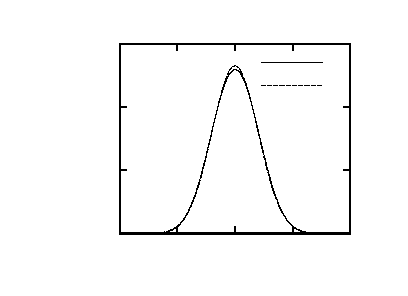
\includegraphics{conv_6}}%

      \put(500,5600){\makebox(0,0)[r]{\strut{}$\mathbf{n=1}$}}%
      \put(858,3440){\makebox(0,0)[r]{\strut{} 0}}%
      \put(858,4045){\makebox(0,0)[r]{\strut{} 0.15}}%
      \put(858,4651){\makebox(0,0)[r]{\strut{} 0.3}}%
      \put(858,5256){\makebox(0,0)[r]{\strut{} 0.45}}%
      \put(990,3220){\makebox(0,0){\strut{}-5}}%
      \put(1543,3220){\makebox(0,0){\strut{}-2.5}}%
      \put(2097,3220){\makebox(0,0){\strut{} 0}}%
      \put(2650,3220){\makebox(0,0){\strut{} 2.5}}%
      \put(3203,3220){\makebox(0,0){\strut{} 5}}%
      \put(1100,5083){\makebox(0,0)[l]{\strut{}sum}}%
      \put(1100,4863){\makebox(0,0)[l]{\strut{}gaussian}}%
          \put(0,3000){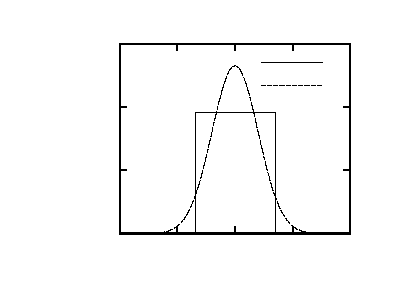
\includegraphics{conv_0}}%

      \put(4500,5600){\makebox(0,0)[r]{\strut{}$\mathbf{n=2}$}}%
      \put(4858,3440){\makebox(0,0)[r]{\strut{} 0}}%
      \put(4858,4045){\makebox(0,0)[r]{\strut{} 0.15}}%
      \put(4858,4651){\makebox(0,0)[r]{\strut{} 0.3}}%
      \put(4858,5256){\makebox(0,0)[r]{\strut{} 0.45}}%
      \put(4990,3220){\makebox(0,0){\strut{}-5}}%
      \put(5543,3220){\makebox(0,0){\strut{}-2.5}}%
      \put(6097,3220){\makebox(0,0){\strut{} 0}}%
      \put(6650,3220){\makebox(0,0){\strut{} 2.5}}%
      \put(7203,3220){\makebox(0,0){\strut{} 5}}%
      \put(5100,5083){\makebox(0,0)[l]{\strut{}sum}}%
      \put(5100,4863){\makebox(0,0)[l]{\strut{}gaussian}}%
          \put(4000,3000){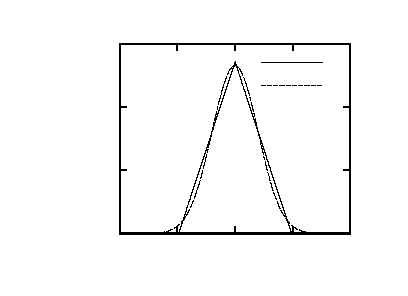
\includegraphics{conv_1}}%



  \end{picture}%
\endgroup

\end{center}
\caption{$U_n$ for different $n$s where $X$ is the uniform distribution.\label{fig_const}}
\end{figure}

We won't prove the central limit theorem here, doing so involves a bit
of detail in deciding what we mean by \lq{}for $n$ approaching
infinity\rq{}. The proof itself involves some messing about with the
moment generating theorem which we haven't studied, but otherwise
isn't too hard. It isn't particularly revealing though; it misses what
is happening, which is roughly this: the central limit theorem is a
bit like the binomial distribution, just like the binomial
distribution quantifies the different ways to get different numbers of
$S$, the central limit theorem quantifies different ways of getting
the same sum. In fact, numerically, the Gau\ss{}ian distribution is
close to the binomial distribution, see for example
Fig.~\ref{fig_binomial}.


\begin{figure}[tb]
\begin{center}
% GNUPLOT: LaTeX picture with Postscript
\begingroup
  \makeatletter
  \providecommand\color[2][]{%
    \GenericError{(gnuplot) \space\space\space\@spaces}{%
      Package color not loaded in conjunction with
      terminal option `colourtext'%
    }{See the gnuplot documentation for explanation.%
    }{Either use 'blacktext' in gnuplot or load the package
      color.sty in LaTeX.}%
    \renewcommand\color[2][]{}%
  }%
  \providecommand\includegraphics[2][]{%
    \GenericError{(gnuplot) \space\space\space\@spaces}{%
      Package graphicx or graphics not loaded%
    }{See the gnuplot documentation for explanation.%
    }{The gnuplot epslatex terminal needs graphicx.sty or graphics.sty.}%
    \renewcommand\includegraphics[2][]{}%
  }%
  \providecommand\rotatebox[2]{#2}%
  \@ifundefined{ifGPcolor}{%
    \newif\ifGPcolor
    \GPcolorfalse
  }{}%
  \@ifundefined{ifGPblacktext}{%
    \newif\ifGPblacktext
    \GPblacktexttrue
  }{}%
  % define a \g@addto@macro without @ in the name:
  \let\gplgaddtomacro\g@addto@macro
  % define empty templates for all commands taking text:
  \gdef\gplbacktext{}%
  \gdef\gplfronttext{}%
  \makeatother
  \ifGPblacktext
    % no textcolor at all
    \def\colorrgb#1{}%
    \def\colorgray#1{}%
  \else
    % gray or color?
    \ifGPcolor
      \def\colorrgb#1{\color[rgb]{#1}}%
      \def\colorgray#1{\color[gray]{#1}}%
      \expandafter\def\csname LTw\endcsname{\color{white}}%
      \expandafter\def\csname LTb\endcsname{\color{black}}%
      \expandafter\def\csname LTa\endcsname{\color{black}}%
      \expandafter\def\csname LT0\endcsname{\color[rgb]{1,0,0}}%
      \expandafter\def\csname LT1\endcsname{\color[rgb]{0,1,0}}%
      \expandafter\def\csname LT2\endcsname{\color[rgb]{0,0,1}}%
      \expandafter\def\csname LT3\endcsname{\color[rgb]{1,0,1}}%
      \expandafter\def\csname LT4\endcsname{\color[rgb]{0,1,1}}%
      \expandafter\def\csname LT5\endcsname{\color[rgb]{1,1,0}}%
      \expandafter\def\csname LT6\endcsname{\color[rgb]{0,0,0}}%
      \expandafter\def\csname LT7\endcsname{\color[rgb]{1,0.3,0}}%
      \expandafter\def\csname LT8\endcsname{\color[rgb]{0.5,0.5,0.5}}%
    \else
      % gray
      \def\colorrgb#1{\color{black}}%
      \def\colorgray#1{\color[gray]{#1}}%
      \expandafter\def\csname LTw\endcsname{\color{white}}%
      \expandafter\def\csname LTb\endcsname{\color{black}}%
      \expandafter\def\csname LTa\endcsname{\color{black}}%
      \expandafter\def\csname LT0\endcsname{\color{black}}%
      \expandafter\def\csname LT1\endcsname{\color{black}}%
      \expandafter\def\csname LT2\endcsname{\color{black}}%
      \expandafter\def\csname LT3\endcsname{\color{black}}%
      \expandafter\def\csname LT4\endcsname{\color{black}}%
      \expandafter\def\csname LT5\endcsname{\color{black}}%
      \expandafter\def\csname LT6\endcsname{\color{black}}%
      \expandafter\def\csname LT7\endcsname{\color{black}}%
      \expandafter\def\csname LT8\endcsname{\color{black}}%
    \fi
  \fi
  \setlength{\unitlength}{0.0500bp}%
  \begin{picture}(5040.00,3528.00)%
    \gplgaddtomacro\gplbacktext{%
      \csname LTb\endcsname%
      \put(990,440){\makebox(0,0)[r]{\strut{} 0}}%
      \put(990,864){\makebox(0,0)[r]{\strut{} 0.025}}%
      \put(990,1289){\makebox(0,0)[r]{\strut{} 0.05}}%
      \put(990,1714){\makebox(0,0)[r]{\strut{} 0.075}}%
      \put(990,2138){\makebox(0,0)[r]{\strut{} 0.1}}%
      \put(990,2563){\makebox(0,0)[r]{\strut{} 0.125}}%
      \put(990,2987){\makebox(0,0)[r]{\strut{} 0.15}}%
      \put(1122,220){\makebox(0,0){\strut{} 0}}%
      \put(1513,220){\makebox(0,0){\strut{} 2}}%
      \put(1904,220){\makebox(0,0){\strut{} 4}}%
      \put(2296,220){\makebox(0,0){\strut{} 6}}%
      \put(2687,220){\makebox(0,0){\strut{} 8}}%
      \put(3078,220){\makebox(0,0){\strut{} 10}}%
      \put(3469,220){\makebox(0,0){\strut{} 12}}%
      \put(3861,220){\makebox(0,0){\strut{} 14}}%
      \put(4252,220){\makebox(0,0){\strut{} 16}}%
      \put(4643,220){\makebox(0,0){\strut{} 18}}%
    }%
    \gplgaddtomacro\gplfronttext{%
      \csname LTb\endcsname%
      \put(3656,3090){\makebox(0,0)[r]{\strut{}$p$=0.25}}%
      \csname LTb\endcsname%
      \put(3656,2870){\makebox(0,0)[r]{\strut{}gaussian}}%
    }%
    \gplbacktext
    \put(0,0){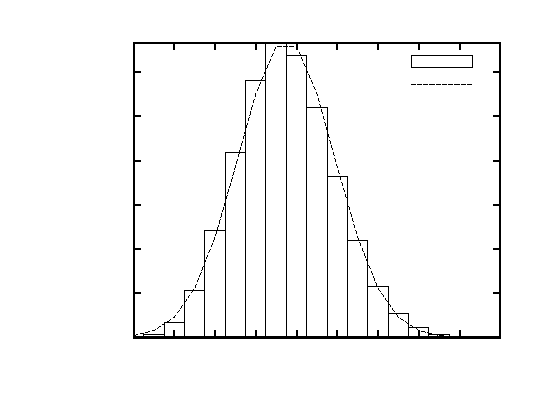
\includegraphics{binomial}}%
    \gplfronttext
  \end{picture}%
\endgroup

\end{center}
\caption{This compares the binomial distribution with $n=30$ and
  $p=0.25$ with the  Gau\ss{}ian distribution with the same mean and variance.\label{fig_binomial}}
\end{figure}


The central limit theorem is important in two ways. First off, it
tells us how the sample mean behaves; since we often estimate means by
doing multiple independent trials this is useful. The second point is
vaguer, although we have stated the central limit theorem in terms of
i.i.d. variables and this is the case where it is easy to state and
prove the theorem, there is a more general phenomena, which is that if
you add independent variables, even if they are not identical, then
the result is a Gau\ss{}ian. This is why so many things show
Gau\ss{}ian distributions. Think, for example, of the height of trees,
lots of things contribute to the height of a tree, how wet and sunny
the location it is growing in, the soil, the genetics of each
individual. These individual contributions probably aren't
Gau\ss{}ian, they aren't identical and, in fact, probably don't
contribute in a linear way to the height, nonetheless we would expect
the result, the height of the trees to be Gau\ss{}ian. It is a
fortunate aspect of statistics, things that are complicated and have
multiple contributing factors, tend to behave in a simple way from the
point-of-view of statistics.


\ifind
\section*{Summary}
\else
\subsection*{1 Probability theory}
\fi

\begin{itemize}
\item A \textbf{sample space} is a set of point, they are the possible \textbf{outcomes} of a \textbf{trial}.
\item An \textbf{event} is a subset of a sample space.
\item A \textbf{probability} is a map from events to real numbers such that
  \begin{enumerate}
    \item $P(A)\ge 0$ for all events.
    \item $P(X)=1$
    \item If $A\cap B=\emptyset$ for two events $A$ and $B$ then 
      \begin{equation}
        P(A\cup B)=P(A)+P(B)
      \end{equation}
\end{enumerate}
\item A \textbf{probability mass function} is a map from points in the sample space to real numbers such that
  \begin{enumerate}
\item $p(x)\ge 0$ for all $x\in X$
\item $\sum_{x\in X} p(x)=1$
  \end{enumerate}
\item $P(A)=\sum_{x\in A}p(x)$
\item If all the points in a sample space have the same probability then
  \begin{equation}
P(A)=\frac{\mbox{number of points in }A}{\mbox{number of points in }X}=\frac{\#A}{\#{X}}
  \end{equation}
  where $\#(A)$ means the number of points in $A$.
  \item The \textbf{binomial coefficient}
\begin{equation}
\left(\begin{array}{c}n\\r\end{array}\right)=\frac{n!}{r!(n-r)!}
\end{equation}
counts the number of subsets of size $r$ in a set of $n$ objects and 
\begin{equation}
n!=n\times (n-1)\times (n-2)\times \ldots \times 2 \times 1
\end{equation}
\end{itemize}



\ifind
\section*{Example question}
\else
\subsection*{6 poisson distribution - example question}
\fi
500 meteorites reach the surface of the Earth each year; what is the
chance of five meteorites reaching the surface in a single day.

\noindent \textbf{solution} Well $\lambda=500/365.25$ and so the probability is
\begin{equation}
p(R=5)=\left(\frac{500}{365.25}\right)^5\frac{1}{5!}e^{-500/365.25}\approx 0.01
\end{equation}



\end{document}




